\chapter{Validate And Adapt Packed Bijou Cell Receipts}\label{record-022}

\noindent{\footnotesize\color{BookMuted}\path{docs/reference/packed-bijou-cells.md}\par}\smallskip

Use \texttt{p\allowbreak{}a\allowbreak{}r\allowbreak{}s\allowbreak{}e\allowbreak{}P\allowbreak{}a\allowbreak{}c\allowbreak{}k\allowbreak{}e\allowbreak{}d\allowbreak{}B\allowbreak{}i\allowbreak{}j\allowbreak{}o\allowbreak{}u\allowbreak{}C\allowbreak{}e\allowbreak{}l\allowbreak{}l\allowbreak{}s\allowbreak{}R\allowbreak{}e\allowbreak{}c\allowbreak{}e\allowbreak{}i\allowbreak{}p\allowbreak{}t\allowbreak{}(\allowbreak{})} to validate an unknown \texttt{p\allowbreak{}a\allowbreak{}c\allowbreak{}k\allowbreak{}e\allowbreak{}d\allowbreak{}-\allowbreak{}b\allowbreak{}i\allowbreak{}j\allowbreak{}o\allowbreak{}u\allowbreak{}-\allowbreak{}c\allowbreak{}e\allowbreak{}l\allowbreak{}l\allowbreak{}s\allowbreak{}/\allowbreak{}1} value. Use \texttt{a\allowbreak{}d\allowbreak{}a\allowbreak{}p\allowbreak{}t\allowbreak{}P\allowbreak{}a\allowbreak{}c\allowbreak{}k\allowbreak{}e\allowbreak{}d\allowbreak{}B\allowbreak{}i\allowbreak{}j\allowbreak{}o\allowbreak{}u\allowbreak{}C\allowbreak{}e\allowbreak{}l\allowbreak{}l\allowbreak{}s\allowbreak{}T\allowbreak{}o\allowbreak{}S\allowbreak{}u\allowbreak{}r\allowbreak{}f\allowbreak{}a\allowbreak{}c\allowbreak{}e\allowbreak{}(\allowbreak{})} when the validated bytes must become a Bijou terminal \texttt{S\allowbreak{}u\allowbreak{}r\allowbreak{}f\allowbreak{}a\allowbreak{}c\allowbreak{}e}.

The adapter preserves the receipt's dimensions, ten-byte cell records, and grapheme side-table order. It does not normalize malformed input, reconstruct cells, render a terminal frame, or validate the complete source scene.

\section{Public API}\label{record-022-public-api}

The package exports:

\begin{center}
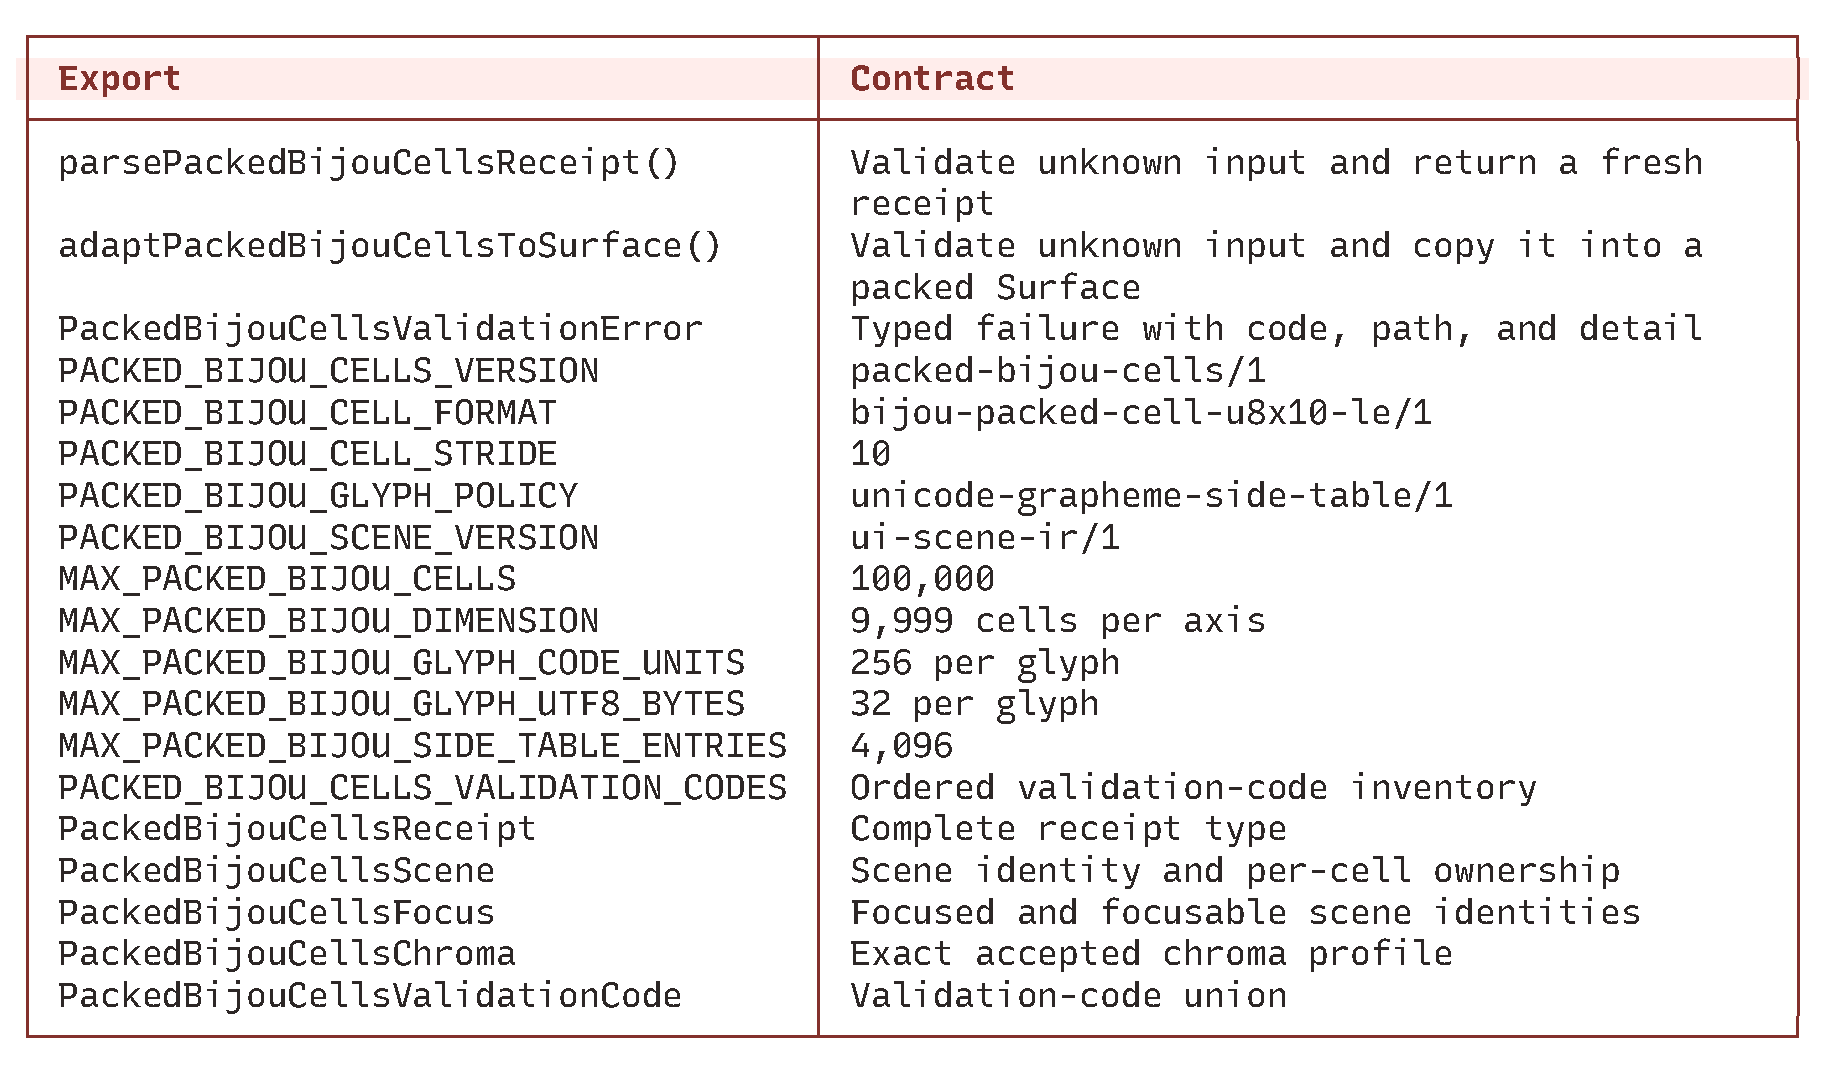
\includegraphics[width=\linewidth]{figures/tables/table-009-g1-1.pdf}
\par\smallskip{\scriptsize\color{BookMuted}Rows 1–19. Actual Bijou table component.}
\end{center}


Import the functions and receipt type from \texttt{@\allowbreak{}f\allowbreak{}l\allowbreak{}y\allowbreak{}i\allowbreak{}n\allowbreak{}g\allowbreak{}r\allowbreak{}o\allowbreak{}b\allowbreak{}o\allowbreak{}t\allowbreak{}s\allowbreak{}/\allowbreak{}b\allowbreak{}i\allowbreak{}j\allowbreak{}o\allowbreak{}u}:

\begin{CodeBlock}
import {
  adaptPackedBijouCellsToSurface,
  parsePackedBijouCellsReceipt,
  type PackedBijouCellsReceipt,
} from '@flyingrobots/bijou';
\end{CodeBlock}

Validate unknown input without constructing a \texttt{S\allowbreak{}u\allowbreak{}r\allowbreak{}f\allowbreak{}a\allowbreak{}c\allowbreak{}e}:

\begin{CodeBlock}
export function validateReceipt(
  input: unknown,
): PackedBijouCellsReceipt {
  return parsePackedBijouCellsReceipt(input);
}
\end{CodeBlock}

Adapt unknown input after validation:

\begin{CodeBlock}
export function adaptReceipt(input: unknown) {
  return adaptPackedBijouCellsToSurface(input);
}
\end{CodeBlock}

Both functions reject invalid input with \texttt{P\allowbreak{}a\allowbreak{}c\allowbreak{}k\allowbreak{}e\allowbreak{}d\allowbreak{}B\allowbreak{}i\allowbreak{}j\allowbreak{}o\allowbreak{}u\allowbreak{}C\allowbreak{}e\allowbreak{}l\allowbreak{}l\allowbreak{}s\allowbreak{}V\allowbreak{}a\allowbreak{}l\allowbreak{}i\allowbreak{}d\allowbreak{}a\allowbreak{}t\allowbreak{}i\allowbreak{}o\allowbreak{}n\allowbreak{}E\allowbreak{}r\allowbreak{}r\allowbreak{}o\allowbreak{}r}. Inspect its \texttt{c\allowbreak{}o\allowbreak{}d\allowbreak{}e}, \texttt{p\allowbreak{}a\allowbreak{}t\allowbreak{}h}, and \texttt{d\allowbreak{}e\allowbreak{}t\allowbreak{}a\allowbreak{}i\allowbreak{}l} fields instead of parsing the message.

\section{Receipt Shape}\label{record-022-receipt-shape}

Every field is required. Unknown or non-enumerable fields, accessors, symbols, sparse arrays, and non-JSON-shaped objects are rejected.

\begin{CodeBlock}
interface PackedBijouCellsReceipt {
  readonly receiptVersion: 'packed-bijou-cells/1';
  readonly widthCells: number;
  readonly heightCells: number;
  readonly cellFormatId: 'bijou-packed-cell-u8x10-le/1';
  readonly glyphPolicyId: 'unicode-grapheme-side-table/1';
  readonly bytes: readonly number[];
  readonly sideTable: readonly string[];
  readonly scene: {
    readonly sceneVersion: 'ui-scene-ir/1';
    readonly sceneHash: string;
    readonly nodeIds: readonly string[];
    readonly cellNodeIds: readonly string[];
  };
  readonly focus: {
    readonly focusedNodeId: string | null;
    readonly focusableNodeIds: readonly string[];
  };
  readonly chroma: {
    readonly colorSpace: 'srgb';
    readonly channelEncoding: 'uint8';
    readonly alphaEncoding: 'uint6';
    readonly terminalDefaultEncoding: 'presence-bits';
  };
}
\end{CodeBlock}

The maximum accepted receipt contains \texttt{1\allowbreak{}0\allowbreak{}0\allowbreak{},\allowbreak{}0\allowbreak{}0\allowbreak{}0} cells, with no axis longer than \texttt{9\allowbreak{},\allowbreak{}9\allowbreak{}9\allowbreak{}9} cells. The byte payload must contain exactly ten unsigned bytes per cell. Negative zero is not a canonical unsigned byte and is rejected.

\section{Cell And Glyph Rules}\label{record-022-cell-and-glyph-rules}

\texttt{c\allowbreak{}e\allowbreak{}l\allowbreak{}l\allowbreak{}F\allowbreak{}o\allowbreak{}r\allowbreak{}m\allowbreak{}a\allowbreak{}t\allowbreak{}I\allowbreak{}d} fixes each cell at ten bytes:

\begin{center}
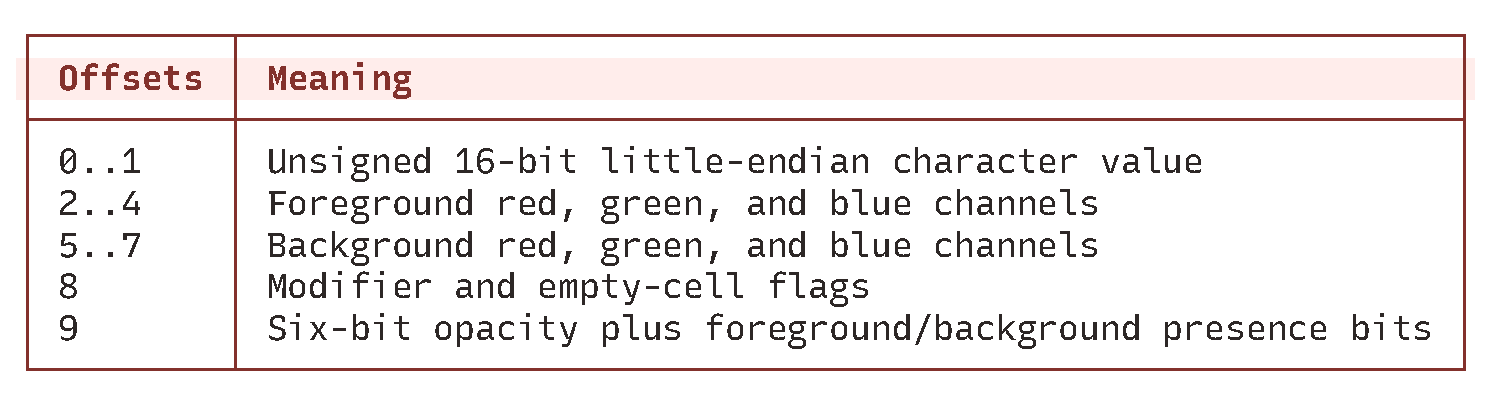
\includegraphics[width=\linewidth]{figures/tables/table-010-g1-1.pdf}
\par\smallskip{\scriptsize\color{BookMuted}Rows 1–5. Actual Bijou table component.}
\end{center}


Character values below \texttt{0\allowbreak{}x\allowbreak{}F\allowbreak{}0\allowbreak{}0\allowbreak{}0} are direct Basic Multilingual Plane values. Direct values must be terminal-control safe and have terminal width \texttt{1}; UTF-16 surrogate values and the NUL sentinel are rejected. An empty cell uses a space glyph plus the empty-cell flag. Values at or above \texttt{0\allowbreak{}x\allowbreak{}F\allowbreak{}0\allowbreak{}0\allowbreak{}0} select \texttt{s\allowbreak{}i\allowbreak{}d\allowbreak{}e\allowbreak{}T\allowbreak{}a\allowbreak{}b\allowbreak{}l\allowbreak{}e\allowbreak{}[\allowbreak{}c\allowbreak{}h\allowbreak{}a\allowbreak{}r\allowbreak{}a\allowbreak{}c\allowbreak{}t\allowbreak{}e\allowbreak{}r\allowbreak{}V\allowbreak{}a\allowbreak{}l\allowbreak{}u\allowbreak{}e\allowbreak{} \allowbreak{}-\allowbreak{} \allowbreak{}0\allowbreak{}x\allowbreak{}F\allowbreak{}0\allowbreak{}0\allowbreak{}0\allowbreak{}]}.

Each side-table entry must be unique, terminal-control safe, and exactly one grapheme with terminal width \texttt{1}. An entry contains at most \texttt{2\allowbreak{}5\allowbreak{}6} UTF-16 code units and encodes to at most \texttt{3\allowbreak{}2} UTF-8 bytes. Format-control, mark-only, and default-ignorable-only graphemes are rejected. Every entry must be referenced by at least one cell. A directly encodable value below \texttt{0\allowbreak{}x\allowbreak{}F\allowbreak{}0\allowbreak{}0\allowbreak{}0} is rejected from the side table. Side-table order is authoritative.

When a foreground or background presence bit is unset, the corresponding three color channels must be zero. An absent color means terminal default, not black. A dashed flag is valid only with the dotted/dashed underline bits.

\section{Scene, Focus, And Chroma Rules}\label{record-022-scene-focus-and-chroma-rules}

\texttt{s\allowbreak{}c\allowbreak{}e\allowbreak{}n\allowbreak{}e\allowbreak{}.\allowbreak{}s\allowbreak{}c\allowbreak{}e\allowbreak{}n\allowbreak{}e\allowbreak{}H\allowbreak{}a\allowbreak{}s\allowbreak{}h} is a lowercase SHA-256 hexadecimal digest. \texttt{s\allowbreak{}c\allowbreak{}e\allowbreak{}n\allowbreak{}e\allowbreak{}.\allowbreak{}n\allowbreak{}o\allowbreak{}d\allowbreak{}e\allowbreak{}I\allowbreak{}d\allowbreak{}s} is a unique non-empty inventory, and \texttt{s\allowbreak{}c\allowbreak{}e\allowbreak{}n\allowbreak{}e\allowbreak{}.\allowbreak{}c\allowbreak{}e\allowbreak{}l\allowbreak{}l\allowbreak{}N\allowbreak{}o\allowbreak{}d\allowbreak{}e\allowbreak{}I\allowbreak{}d\allowbreak{}s} contains one declared owner for every cell.

Every focusable node must occur in \texttt{s\allowbreak{}c\allowbreak{}e\allowbreak{}n\allowbreak{}e\allowbreak{}.\allowbreak{}n\allowbreak{}o\allowbreak{}d\allowbreak{}e\allowbreak{}I\allowbreak{}d\allowbreak{}s}. \texttt{f\allowbreak{}o\allowbreak{}c\allowbreak{}u\allowbreak{}s\allowbreak{}e\allowbreak{}d\allowbreak{}N\allowbreak{}o\allowbreak{}d\allowbreak{}e\allowbreak{}I\allowbreak{}d} is either \texttt{n\allowbreak{}u\allowbreak{}l\allowbreak{}l} or a member of \texttt{f\allowbreak{}o\allowbreak{}c\allowbreak{}u\allowbreak{}s\allowbreak{}a\allowbreak{}b\allowbreak{}l\allowbreak{}e\allowbreak{}N\allowbreak{}o\allowbreak{}d\allowbreak{}e\allowbreak{}I\allowbreak{}d\allowbreak{}s}.

Version \texttt{1} accepts only this chroma profile:

\begin{CodeBlock}
colorSpace: srgb
channelEncoding: uint8
alphaEncoding: uint6
terminalDefaultEncoding: presence-bits
\end{CodeBlock}

No color-space or channel conversion occurs.

\section{Diagnostics}\label{record-022-diagnostics}

The deterministic message format is:

\begin{CodeBlock}
packed-bijou-cells/1 <code> at <path>: <detail>
\end{CodeBlock}

Paths escape control and default-ignorable characters as Unicode escape sequences so diagnostics remain visually stable.

\begin{center}
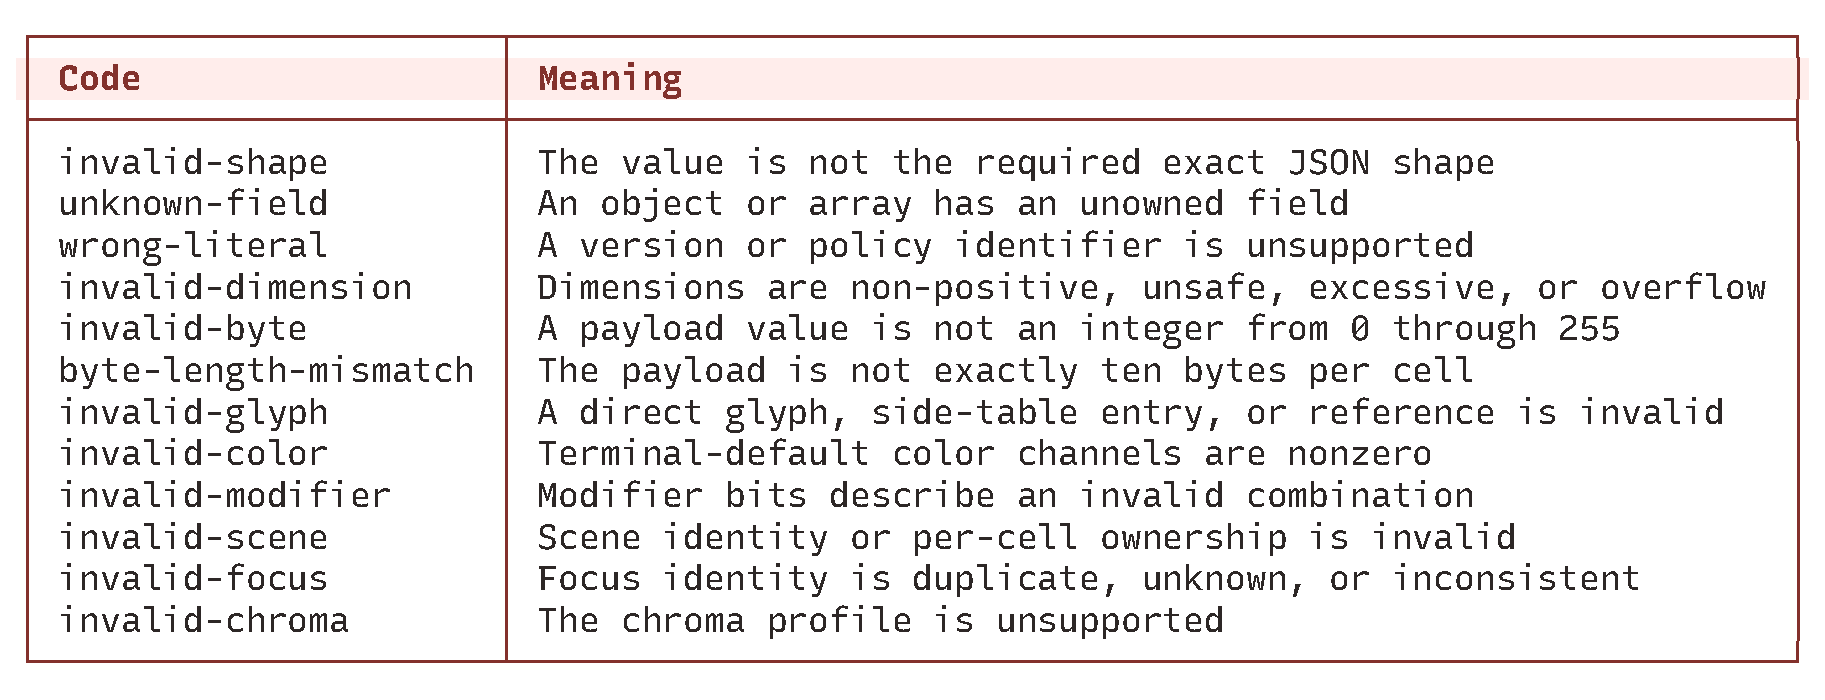
\includegraphics[width=\linewidth]{figures/tables/table-011-g1-1.pdf}
\par\smallskip{\scriptsize\color{BookMuted}Rows 1–12. Actual Bijou table component.}
\end{center}


Paths identify the rejected location, for example \texttt{\$\allowbreak{}.\allowbreak{}b\allowbreak{}y\allowbreak{}t\allowbreak{}e\allowbreak{}s\allowbreak{}[\allowbreak{}1\allowbreak{}7\allowbreak{}]} or \texttt{\$\allowbreak{}.\allowbreak{}f\allowbreak{}o\allowbreak{}c\allowbreak{}u\allowbreak{}s\allowbreak{}.\allowbreak{}f\allowbreak{}o\allowbreak{}c\allowbreak{}u\allowbreak{}s\allowbreak{}e\allowbreak{}d\allowbreak{}N\allowbreak{}o\allowbreak{}d\allowbreak{}e\allowbreak{}I\allowbreak{}d}.

\section{Adapter Result}\label{record-022-adapter-result}

\texttt{a\allowbreak{}d\allowbreak{}a\allowbreak{}p\allowbreak{}t\allowbreak{}P\allowbreak{}a\allowbreak{}c\allowbreak{}k\allowbreak{}e\allowbreak{}d\allowbreak{}B\allowbreak{}i\allowbreak{}j\allowbreak{}o\allowbreak{}u\allowbreak{}C\allowbreak{}e\allowbreak{}l\allowbreak{}l\allowbreak{}s\allowbreak{}T\allowbreak{}o\allowbreak{}S\allowbreak{}u\allowbreak{}r\allowbreak{}f\allowbreak{}a\allowbreak{}c\allowbreak{}e\allowbreak{}(\allowbreak{})} validates the complete receipt before it calls \texttt{c\allowbreak{}r\allowbreak{}e\allowbreak{}a\allowbreak{}t\allowbreak{}e\allowbreak{}S\allowbreak{}u\allowbreak{}r\allowbreak{}f\allowbreak{}a\allowbreak{}c\allowbreak{}e\allowbreak{}(\allowbreak{})}. On success:

\begin{CodeBlock}
surface.width === receipt.widthCells
surface.height === receipt.heightCells
Array.from(surface.buffer) deep-equals receipt.bytes
surface.sideTable deep-equals receipt.sideTable
\end{CodeBlock}

All surface cells are marked dirty for their first render. Scene, focus, and chroma metadata remain receipt evidence; they are not stored inside \texttt{S\allowbreak{}u\allowbreak{}r\allowbreak{}f\allowbreak{}a\allowbreak{}c\allowbreak{}e}.

\section{Fixture And Verification}\label{record-022-fixture-and-verification}

The checked fixture exercises direct glyphs, side-table glyphs, explicit and terminal-default colors, scene ownership, and focus:

\begin{itemize}
\tightlist
\item
  \href{https://github.com/flyingrobots/bijou/blob/cbd70612140e7a450d764b3c7be1c6af878b99bc/tests/fixtures/RE-036/packed-bijou-cells.v1.json}{Packed Bijou cell fixture}
\item
  \href{https://github.com/flyingrobots/bijou/blob/cbd70612140e7a450d764b3c7be1c6af878b99bc/docs/design/RE-036-packed-bijou-cells-surface-adapter.md}{RE-036 design record}
\end{itemize}

Run the focused contract evidence:

\begin{CodeBlock}
npx vitest run tests/cycles/RE-036
\end{CodeBlock}

